% NightShift, journal version (Elsevier elsarticle; target: Future Generation Computer Systems).
% Build from this directory:  latexmk -pdf main.tex
% Numbers come from ../numbers.tex (sim/make_numbers.py) and model_numbers.tex
% (sim/journal_numbers.py). Values printed in blue by \Pending{} are waiting for
% the real-phone measurements of Study A (bench/STUDY.md) and must all be
% replaced before submission (grep -n Pending main.tex lists them).
\documentclass[preprint,review,12pt,authoryear]{elsarticle}
\usepackage{amsmath,amssymb}
\usepackage{booktabs}
\usepackage{microtype}
\usepackage{graphicx}
\usepackage{xcolor}
\usepackage{xurl}
\usepackage{lineno}
\usepackage[hidelinks]{hyperref}
\graphicspath{{../figures/}}
% generated by sim/make_numbers.py; do not edit
\newcommand{\ActCA}{47}
\newcommand{\ActConsol}{44}
\newcommand{\ActLifetime}{50}
\newcommand{\ActNS}{26}
\newcommand{\ActNSNoWait}{46}
\newcommand{\ActReplay}{48}
\newcommand{\ActRestart}{0}
\newcommand{\ActStandby}{50}
\newcommand{\ActSticky}{48}
\newcommand{\ActWait}{51}
\newcommand{\CAvsReplayPct}{+2}
\newcommand{\CIConsCA}{1.7}
\newcommand{\CIConsConsol}{0.0}
\newcommand{\CIConsLifetime}{1.7}
\newcommand{\CIConsNS}{4.0}
\newcommand{\CIConsNSNoWait}{2.7}
\newcommand{\CIConsReplay}{1.7}
\newcommand{\CIConsRestart}{2.0}
\newcommand{\CIConsStandby}{2.5}
\newcommand{\CIConsSticky}{2.2}
\newcommand{\CIConsWait}{2.0}
\newcommand{\CIRepCA}{1.3}
\newcommand{\CIRepConsol}{1.7}
\newcommand{\CIRepLifetime}{1.4}
\newcommand{\CIRepNS}{5.1}
\newcommand{\CIRepNSNoWait}{4.0}
\newcommand{\CIRepReplay}{0.0}
\newcommand{\CIRepRestart}{0.4}
\newcommand{\CIRepStandby}{1.3}
\newcommand{\CIRepSticky}{2.8}
\newcommand{\CIRepWait}{3.5}
\newcommand{\CacheFullCA}{207}
\newcommand{\CacheFullConsol}{182}
\newcommand{\CacheFullNS}{40}
\newcommand{\CacheFullRatioCA}{5}
\newcommand{\CacheFullReplay}{213}
\newcommand{\CacheFullTputCA}{115}
\newcommand{\CacheFullTputConsol}{123}
\newcommand{\CacheFullTputNS}{109}
\newcommand{\CacheFullTputReplay}{114}
\newcommand{\ConsolGainPct}{+8}
\newcommand{\DiffConsCA}{-6.8}
\newcommand{\DiffConsConsol}{+0.0}
\newcommand{\DiffConsLifetime}{-13.2}
\newcommand{\DiffConsNS}{-6.0}
\newcommand{\DiffConsNSNoWait}{-14.8}
\newcommand{\DiffConsReplay}{-8.5}
\newcommand{\DiffConsRestart}{-12.2}
\newcommand{\DiffConsStandby}{-50.4}
\newcommand{\DiffConsSticky}{-20.0}
\newcommand{\DiffConsWait}{-21.6}
\newcommand{\DiffRepCA}{+1.7}
\newcommand{\DiffRepConsol}{+8.5}
\newcommand{\DiffRepLifetime}{-4.8}
\newcommand{\DiffRepNS}{+2.4}
\newcommand{\DiffRepNSNoWait}{-6.4}
\newcommand{\DiffRepReplay}{+0.0}
\newcommand{\DiffRepRestart}{-3.8}
\newcommand{\DiffRepStandby}{-41.9}
\newcommand{\DiffRepSticky}{-11.6}
\newcommand{\DiffRepWait}{-13.1}
\newcommand{\EligiblePct}{90}
\newcommand{\FailCA}{1490}
\newcommand{\FailConsol}{1452}
\newcommand{\FailDropPct}{46}
\newcommand{\FailLifetime}{1469}
\newcommand{\FailNS}{804}
\newcommand{\FailNSNoWait}{1257}
\newcommand{\FailReplay}{1487}
\newcommand{\FailRestart}{1487}
\newcommand{\FailStandby}{859}
\newcommand{\FailSticky}{1285}
\newcommand{\FailWait}{1314}
\newcommand{\GBCA}{363}
\newcommand{\GBConsol}{368}
\newcommand{\GBLifetime}{610}
\newcommand{\GBNS}{57}
\newcommand{\GBNSNoWait}{320}
\newcommand{\GBRatio}{7}
\newcommand{\GBRatioCA}{6}
\newcommand{\GBRatioConsol}{7}
\newcommand{\GBRatioMax}{12}
\newcommand{\GBRatioMin}{2}
\newcommand{\GBReplay}{410}
\newcommand{\GBRestart}{375}
\newcommand{\GBStandby}{492}
\newcommand{\GBSticky}{296}
\newcommand{\GBWait}{302}
\newcommand{\JCA}{7}
\newcommand{\JConsol}{6}
\newcommand{\JLifetime}{7}
\newcommand{\JNS}{6}
\newcommand{\JNSNoWait}{6}
\newcommand{\JReplay}{7}
\newcommand{\JRestart}{7}
\newcommand{\JStandby}{6}
\newcommand{\JSticky}{7}
\newcommand{\JWait}{7}
\newcommand{\LatCA}{2.3}
\newcommand{\LatConsol}{2.3}
\newcommand{\LatLAN}{2.0}
\newcommand{\LatLifetime}{2.3}
\newcommand{\LatNS}{2.3}
\newcommand{\LatNSNoWait}{2.3}
\newcommand{\LatReplay}{2.3}
\newcommand{\LatRestart}{2.3}
\newcommand{\LatSlow}{3.2}
\newcommand{\LatStandby}{2.3}
\newcommand{\LatSticky}{2.3}
\newcommand{\LatWAN}{2.3}
\newcommand{\LatWait}{2.3}
\newcommand{\MinAvail}{35}
\newcommand{\NPhones}{1{,}000}
\newcommand{\NSbehindConsolPct}{5}
\newcommand{\NSvsCAPct}{+1}
\newcommand{\NSvsConsolPct}{-5}
\newcommand{\NSvsReplayPct}{+2}
\newcommand{\NightSharePct}{98}
\newcommand{\OracleCA}{66}
\newcommand{\OracleConsol}{70}
\newcommand{\OracleLifetime}{62}
\newcommand{\OracleNS}{66}
\newcommand{\OracleNSNoWait}{61}
\newcommand{\OracleReplay}{65}
\newcommand{\OracleRestart}{71}
\newcommand{\OracleStandby}{39}
\newcommand{\OracleSticky}{58}
\newcommand{\OracleWait}{57}
\newcommand{\PeakAvail}{731}
\newcommand{\PeakPipes}{36}
\newcommand{\PhoneGBCA}{4.0}
\newcommand{\PhoneGBConsol}{4.3}
\newcommand{\PhoneGBLifetime}{6.3}
\newcommand{\PhoneGBNS}{0.7}
\newcommand{\PhoneGBNSNoWait}{3.4}
\newcommand{\PhoneGBReplay}{4.4}
\newcommand{\PhoneGBRestart}{3.9}
\newcommand{\PhoneGBStandby}{3.2}
\newcommand{\PhoneGBSticky}{3.0}
\newcommand{\PhoneGBWait}{2.9}
\newcommand{\PoolLargeGBNS}{35}
\newcommand{\PoolLargeGBRatio}{12}
\newcommand{\PoolLargeGBRatioCA}{10}
\newcommand{\PoolLargeGBReplay}{428}
\newcommand{\PoolLargeGainPct}{+17}
\newcommand{\PoolLargeVsConsolPct}{+7}
\newcommand{\PoolSmallGBNS}{162}
\newcommand{\PoolSmallGBRatio}{2}
\newcommand{\PoolSmallGBRatioCA}{2}
\newcommand{\PoolSmallGBReplay}{374}
\newcommand{\PoolSmallGainPct}{-9}
\newcommand{\PoolSmallVsConsolPct}{-14}
\newcommand{\RestartVsReplayPct}{-4}
\newcommand{\Seeds}{5}
\newcommand{\ShardCA}{316}
\newcommand{\ShardConsol}{323}
\newcommand{\ShardLifetime}{561}
\newcommand{\ShardNS}{30}
\newcommand{\ShardNSNoWait}{273}
\newcommand{\ShardRatio}{12}
\newcommand{\ShardReplay}{362}
\newcommand{\ShardRestart}{375}
\newcommand{\ShardStandby}{443}
\newcommand{\ShardSticky}{247}
\newcommand{\ShardWait}{251}
\newcommand{\StandbyDropPct}{39}
\newcommand{\StickyGainPct}{-11}
\newcommand{\SwBatchHiNS}{146}
\newcommand{\SwBatchHiReplay}{145}
\newcommand{\SwBatchLoNS}{61}
\newcommand{\SwBatchLoReplay}{59}
\newcommand{\SwDayDurHiNS}{121}
\newcommand{\SwDayDurHiReplay}{119}
\newcommand{\SwDayDurLoNS}{105}
\newcommand{\SwDayDurLoReplay}{109}
\newcommand{\SwHopHiNS}{76}
\newcommand{\SwHopHiReplay}{75}
\newcommand{\SwHopLoNS}{120}
\newcommand{\SwHopLoReplay}{119}
\newcommand{\SwNightHiNS}{138}
\newcommand{\SwNightHiReplay}{129}
\newcommand{\SwNightLoNS}{58}
\newcommand{\SwNightLoReplay}{63}
\newcommand{\SwPoolHiCA}{110}
\newcommand{\SwPoolHiConsol}{119}
\newcommand{\SwPoolHiNS}{127}
\newcommand{\SwPoolHiReplay}{109}
\newcommand{\SwPoolLoCA}{109}
\newcommand{\SwPoolLoConsol}{115}
\newcommand{\SwPoolLoNS}{98}
\newcommand{\SwPoolLoReplay}{108}
\newcommand{\SwPrefillHiNS}{134}
\newcommand{\SwPrefillHiReplay}{132}
\newcommand{\SwPrefillLoNS}{58}
\newcommand{\SwPrefillLoReplay}{59}
\newcommand{\TputCA}{108}
\newcommand{\TputConsol}{115}
\newcommand{\TputGainPct}{2}
\newcommand{\TputLifetime}{101}
\newcommand{\TputNS}{109}
\newcommand{\TputNSNoWait}{100}
\newcommand{\TputReplay}{106}
\newcommand{\TputRestart}{102}
\newcommand{\TputSDCA}{2.4}
\newcommand{\TputSDConsol}{2.9}
\newcommand{\TputSDLifetime}{2.4}
\newcommand{\TputSDNS}{4.9}
\newcommand{\TputSDNSNoWait}{4.1}
\newcommand{\TputSDReplay}{1.7}
\newcommand{\TputSDRestart}{1.5}
\newcommand{\TputSDStandby}{1.5}
\newcommand{\TputSDSticky}{3.3}
\newcommand{\TputSDWait}{4.1}
\newcommand{\TputStandby}{64}
\newcommand{\TputSticky}{95}
\newcommand{\TputWait}{93}
\newcommand{\UsefulCA}{65}
\newcommand{\UsefulConsol}{70}
\newcommand{\UsefulLifetime}{61}
\newcommand{\UsefulNS}{83}
\newcommand{\UsefulNSNoWait}{69}
\newcommand{\UsefulReplay}{64}
\newcommand{\UsefulRestart}{70}
\newcommand{\UsefulStandby}{74}
\newcommand{\UsefulSticky}{65}
\newcommand{\UsefulWait}{64}
\newcommand{\WaitSixtyGB}{109}
\newcommand{\WaitSixtyTput}{107}
\newcommand{\WaitTenGB}{45}
\newcommand{\WaitTenTput}{108}
\newcommand{\WaitZeroGB}{314}
\newcommand{\WaitZeroTput}{99}
\newcommand{\WaitvsCAPct}{-14}

% generated by sim/journal_numbers.py from sim/results/traffic_model.json
\newcommand{\TMErrAbsMaxPct}{12}
\newcommand{\TMErrAbsMeanPct}{5.6}
\newcommand{\TMErrWorstKey}{NightShift at 2,000 phones}
\newcommand{\TMErrWorstWhy}{downloads are rare (about 99 per run), so a handful of events moves the relative error by several points; among the busier policies the largest error is for Sticky, where the drift balance treats every fallback as equally likely to land on a phone that has not drifted yet}
\newcommand{\TMqSixteenPct}{35.6}
\newcommand{\TMqFortyEightPct}{4.5}
\newcommand{\TMFormPerfect}{5.7}
\newcommand{\TMFormGreedy}{7.6}
\newcommand{\TMFormCacheN}{10}
\newcommand{\TMFormCacheFracPct}{12}


\newcommand{\Pending}[1]{\textcolor{blue}{[#1]}}

\journal{Future Generation Computer Systems}

\begin{document}

\begin{frontmatter}

\title{NightShift: Churn-Tolerant Batch Inference of Large Language Models on Pools of Charging Smartphones}

\author{Aidin Bazarchi}
\affiliation{organization={Independent Researcher}}

\begin{abstract}
Many smartphones spend the night plugged in, on Wi-Fi and idle. We study
whether such a pool can run inference for a large language model (LLM) too big
for any single phone, and what it would take. A 70-billion-parameter model at
4 bits needs about 40\,GB, so one copy of the model is a pipeline of 16 phones,
each of which leaves without warning when its owner unplugs it. We first derive
what such a pool can and cannot do: it is a throughput machine for batch work
with seconds per output token, not a conversational service. We then build a
churn-aware simulator whose phone, network and user parameters are explicit,
replaceable assumptions, and an analytical model of the data traffic that
churn causes, which predicts the simulator's traffic within
\TMErrAbsMaxPct\% across ten scheduling policies and pool sizes from 500 to
4,000 phones. Both show that once phones come and go, the dominant cost of
churn is moving model shards to the phones that replace leavers, not
recomputing lost work: a fair cache-aware baseline downloads \GBCA\,GB per
million tokens, about \PhoneGBCA\,GB per serving phone per day. NightShift
gives every phone a permanent home block, lets a vacant stage wait briefly for
a phone that already holds it, and consolidates broken pipelines. With 1,000
phones it downloads \GBRatioBaseMin--\GBRatioBaseMax$\times$ less data than
each of six baselines, with throughput equal to Petals-style replay within
noise and \NSbehindConsolPct\% below the best baseline; at 4,000 phones it is
ahead on both. Dedicated warm standbys, the usual remedy for failures, cut
throughput by \StandbyDropPct\%. We discuss privacy, integrity, battery wear,
data plans and incentives, report \Pending{Study A: measured per-layer times,
batching cost, hop latency and session statistics from N Android phones}, and
release the simulator, the model and a benchmark kit.
\end{abstract}

\begin{keyword}
large language models \sep distributed inference \sep volunteer computing \sep
smartphones \sep pipeline parallelism \sep churn \sep edge computing
\end{keyword}

\end{frontmatter}

\linenumbers

%% ---------------------------------------------------------------------------
\section{Introduction}
\label{sec:intro}

Volunteer computing has a long record. BOINC and SETI@home turned idle desktops
into a scientific computer~\citep{boinc,anderson2006}, Folding@home did the
same for protein dynamics~\citep{foldingathome}, and Google's federated
learning system trains models on phones only while they are ``idle, charging
and on an unmetered network''~\citep{bonawitz2019}. Large language models now
consume a large and growing share of data-centre compute~\citep{samsi2023,luccioni2024},
which invites a question: could the idle phones of the world run them?

The question has an easy wrong answer in each direction. ``Yes, enough phones
beat any data centre'' ignores that generation is sequential and that a large
model does not fit in a phone. ``No, phones are too small'' ignores that the
same was said of volunteer desktops, and that systems such as
Petals~\citep{petals-acl,petals-neurips} already serve 100B-class models from
pipelines of volunteer GPUs over the internet. The interesting question is
quantitative: \emph{for which workloads, at what throughput and at what cost to
the volunteers, and which design choices matter?}

Three properties make a pool of phones different from the volunteer GPUs that
Petals targets and from the preemptible cloud instances that
SpotServe~\citep{spotserve} and Bamboo~\citep{bamboo} target. A phone holds a
small slice of a large model, so even one model copy spans many devices.
Phones leave without warning, at a rate that follows their owners' daily lives.
And every byte moved to a phone is paid for by its owner, in data, time and
battery, so data movement is not a free internal cost of the scheduler but the
main thing a volunteer gives up. The last property, we find, decides which
designs are viable.

This paper makes four contributions.
\begin{enumerate}
\item \textbf{A first-principles analysis} (Section~\ref{sec:physics}) of what
a phone pool can and cannot do. It suits throughput-oriented batch jobs, not
interactive chat, and it reads far more weight memory per token than a GPU, so
its case rests on marginal cost, not efficiency.
\item \textbf{A churn-aware simulator} (Section~\ref{sec:method}) driven by a
diurnal model of when phones are charging and on Wi-Fi. Every phone, network
and user parameter is explicit and can be replaced by a measurement; a
benchmark kit produces those measurements on Android phones
(Section~\ref{sec:measure}).
\item \textbf{An analytical model of shard traffic}
(Section~\ref{sec:model}) that explains where the data a pool downloads comes
from. It treats each scheduling decision as a draw from the idle pool and
predicts the simulator's downloads within \TMErrAbsMaxPct\% for ten policies
at 1,000 phones and for four of them at pool sizes from 500 to 4,000. It shows why matching cached phones, however carefully, cannot remove
most of the traffic when phones keep whatever block they served last, and why a
fixed assignment can.
\item \textbf{NightShift} (Section~\ref{sec:design}), a placement and recovery
design built on that observation: a permanent home block per phone, a short
wait for a phone that holds the vacant block, and consolidation of broken
pipelines. It cuts data downloaded \GBRatioBaseMin--\GBRatioBaseMax$\times$
against six baselines at 1,000 phones, including a fair cache-aware one, and
\CacheFullRatioCA$\times$ against cache-aware even when phones cache the whole
model. Throughput matches replay within noise and is \NSbehindConsolPct\%
below the best baseline at this size; NightShift overtakes that baseline as
the pool grows (from about \PoolCross{} phones) and trails at 500 phones. An
ablation shows that neither the wait nor consolidation helps alone, and that
dedicated standbys make things worse.
\end{enumerate}

We also examine the questions that decide whether such a system should be
deployed at all: the privacy of prompts passing through strangers' phones, the
integrity of their outputs, battery wear and heat, data plans, and incentives
(Section~\ref{sec:security} and Section~\ref{sec:owners}). We are explicit
about what is measured and what is assumed. The design results come from
simulation with stated assumptions (Table~\ref{tab:params});
Section~\ref{sec:measure} reports the measurements that calibrate them and
quantifies how far the simulator's timing model is from a real pipeline of
phones. The simulator, the analytical model, all results and the benchmark kit
are released (see Data availability).

%% ---------------------------------------------------------------------------
\section{The physics of a phone pool}
\label{sec:physics}

This section derives, from a few numbers, the operating regime of a pool of
phones. Table~\ref{tab:params} lists the values; Section~\ref{sec:measure}
replaces them with measurements.

\paragraph{Memory} A 70B model quantised to about 4 bits per
weight~\citep{gptq,awq} occupies roughly 40\,GB; we model 80 layers of
0.5\,GB, the shape of Llama-class models~\citep{llama2,llama3}. An Android app
running in the background can rarely hold more than a fraction of a phone's
RAM; we assume 45\%, so an 8\,GB phone offers 3.6\,GB. With the key--value
(KV) cache for a batch of 32 sequences of 768 tokens, a five-layer block needs
3.0\,GB, so a model copy is a pipeline of $B=16$ phones, and phones with
6\,GB of RAM cannot take part at all (\EligiblePct\% of our pool is
eligible). Smaller blocks would admit more phones but lengthen the pipeline,
which raises both the time per token and the chance that some member leaves.

\paragraph{Time per output token} Generating one token visits all $B$
stages in order. Let $\tau_i$ be the compute time of stage $i$ for one
micro-batch and $h$ the one-way latency of a hop between phones. A token's
\emph{trip} through the pipeline takes $\sum_i \tau_i + B h$. With $B$
micro-batches in flight, a pipeline also cannot finish a round of tokens faster
than $B$ times its slowest stage. The time per output token is therefore
\begin{equation}
T_{\text{tok}} = \max\Bigl(\sum_{i=1}^{B}\tau_i + B h,\; B \max_i \tau_i\Bigr).
\label{eq:ttok}
\end{equation}
At roughly 15\,ms per layer on a mid-range phone (plus 10\% for micro-batches
of two) and 60\,ms per wide-area hop, the trip takes about 1.3\,s of compute
plus 1.0\,s of network, and the slowest stage bound is typically about 2\,s.
Equation~(\ref{eq:ttok}) gives \LatWAN\,s at 60\,ms hops, where the trip
dominates, and still \LatLAN\,s on a household network (5\,ms hops), where the
slowest phone sets the pace and the trip alone would take only \PassLAN\,s.
Speculative decoding~\citep{specdec} or faster phones would shorten this, but
not to the sub-second times a conversational assistant needs.

\paragraph{Throughput} Latency need not limit throughput. With many sequences
in flight, a pipeline keeps every stage busy, as in the micro-batching of
GPipe and PipeDream~\citep{gpipe,pipedream} and in continuous batching
servers~\citep{orca,vllm,sarathi}. A pipeline of $B$ stages that carries $S$
sequences produces $S/T_{\text{tok}}$ tokens per second, about 13 tokens per
second for $S=32$ at our parameters, before losses to churn. Batch workloads such as offline
evaluation, synthetic data generation, document summarisation or embedding a
corpus tolerate hours of latency, the same regime FlexGen targets on a single
GPU~\citep{flexgen}, and providers already sell such work at a discount through
batch interfaces.

\paragraph{Memory traffic and energy} The price is efficiency. A data-centre
GPU serving a batch of 128 reads each weight once per 128 tokens, about
0.3\,GB of weight traffic per token for a 70B model. A phone pipeline with 32
sequences over 16 stages processes micro-batches of two, so it reads about
20\,GB per token, roughly 60$\times$ more. At an assumed 4\,W per active phone
and 1\,W while waiting, the simulated pool spends about \JNS\,J per token,
which is well above published per-token energy figures for GPU
servers~\citep{samsi2023}, although those come from different models and
workloads and are not a like-for-like comparison. The phone pool's argument is
therefore not efficiency but \emph{marginal cost}: the hardware is already
bought, already powered at night and otherwise idle. Whether that argument
survives battery wear and the owner's electricity bill is examined in
Section~\ref{sec:owners}.

\paragraph{Data movement} The last number is the one this paper is about. A
block is 2.5\,GB. At a median residential downlink of 50\,Mbit/s, moving one
block to a phone takes about 7 minutes; reading it from the phone's own flash
takes 2.5\,s. A phone that has to download a block whenever it is recruited
for a different one pays minutes of idle time and gigabytes of its owner's data
each time. How often that happens is a property of the scheduler, and it is
what Section~\ref{sec:model} models.

%% ---------------------------------------------------------------------------
\section{Related work}
\label{sec:related}

\paragraph{Volunteer, desktop-grid and federated computing}
BOINC~\citep{boinc} established redundant execution and work units for
untrusted volunteers, and its projects measured the computational and storage
potential of volunteer hosts~\citep{anderson2006}; surveys summarise the
requirements such systems share~\citep{durrani2014}. Desktop-grid studies
characterised host availability and its effect on scheduling~\citep{kondo2004},
fitted statistical models of availability to SETI@home
hosts~\citep{javadi2009}, and collected failure traces from many distributed
systems~\citep{fta}. These systems ran independent jobs: a host that left lost
only its own work unit. Federated learning~\citep{fedavg,bonawitz2019,kairouz2021}
runs on phones at production scale and established the eligibility rule we
adopt (charging, on Wi-Fi, idle). Participant selection~\citep{oort} and
asynchronous aggregation~\citep{papaya} deal with heterogeneous, intermittently
available clients; device availability has been measured at large
scale~\citep{yang2021heterogeneity,fedscale}, and those traces are natural
inputs to our simulator. In federated learning each phone trains a full small
model; nothing is split across devices, so a departure costs one update, not a
pipeline.

\paragraph{LLMs over unreliable or heterogeneous hardware}
Petals~\citep{petals-acl,petals-neurips} serves large models from pipelines of
volunteer GPUs and recovers from departures by routing around them and
replaying the lost stage's cache; it is the baseline we call \emph{replay}.
SWARM~\citep{swarm}, Learning@home~\citep{learningathome} and
DiLoCo~\citep{diloco} train over unreliable or poorly connected nodes.
Deserve~\citep{deserve} studies decentralised serving on volunteer GPUs;
HexGen~\citep{hexgen} and Helix~\citep{helix} place LLM inference over
heterogeneous GPUs. SpotServe~\citep{spotserve} serves LLMs on preemptible cloud
instances, migrating context when an instance is reclaimed, and
SkyServe~\citep{skyserve} spreads replicas across regions and clouds to survive
spot preemptions. For training, Bamboo~\citep{bamboo} adds redundant
computation and Oobleck~\citep{oobleck} keeps redundant pipeline templates to
survive failures, and Parcae~\citep{parcae} predicts spot-instance
availability to adapt parallelism proactively, the same idea as our lifetime
grouping. Those nodes are GPUs with tens of gigabytes and, often, seconds to
minutes of warning; ours are phones with a few gigabytes and no warning, and
moving a shard to a replacement costs the volunteer data.

\paragraph{Parallelism for LLM serving}
Model and pipeline parallelism~\citep{megatron,gpipe,pipedream} and their
automatic combination~\citep{alpa} are the basis of every multi-device LLM
system. Serving systems batch continuously~\citep{orca}, page the KV
cache~\citep{vllm}, split prefill from decode across
machines~\citep{splitwise,distserve}, chunk prefills to balance latency and
throughput~\citep{sarathi}, and partition large models carefully across
accelerators~\citep{pope2023,dsinference}. They assume a stable set of
well-connected accelerators. We borrow their pipeline arithmetic and keep
their batching, and change the problem: membership changes all the time.

\paragraph{Splitting models across nearby devices}
LinguaLinked~\citep{lingualinked} runs one LLM across several Android phones,
Galaxy~\citep{galaxy} and EdgeShard~\citep{edgeshard} split transformers across
edge devices, exo~\citep{exo} does so for a household's laptops and phones, and
prima.cpp~\citep{primacpp} runs 70B-class models on a home cluster of everyday
devices; a recent survey covers this space~\citep{edgellmsurvey}. Earlier,
MoDNN~\citep{modnn} and DeepThings~\citep{deepthings} split CNNs,
MAUI~\citep{maui} and CloneCloud~\citep{clonecloud} offloaded phone code to the
cloud, and CWC~\citep{cwc} scheduled jobs on the idle, charging phones of an
organisation. Table~\ref{tab:compare} places NightShift among the closest
systems. They assume a small, stable set of devices, typically in one home or
one local network. We study the opposite regime: a large pool in which
membership changes all the time.

\begin{table}[t]
\caption{Closest systems. ``Churn'': devices leave during inference (for
SpotServe, after a short preemption notice). ``Shard traffic'': the cost of moving weights to replacements is
modelled.}
\label{tab:compare}
\small
\begin{tabular}{@{}llll@{}}
\toprule
System & Devices & Churn & Shard traffic\\
\midrule
Petals~\citep{petals-neurips} & volunteer GPUs & yes & no\\
SpotServe~\citep{spotserve} & cloud spot GPUs & with warning & no\\
LinguaLinked~\citep{lingualinked} & phones, one LAN & no & no\\
EdgeShard~\citep{edgeshard} & edge devices & no & no\\
prima.cpp~\citep{primacpp} & home devices & no & no\\
CWC~\citep{cwc} & charging phones & yes & n/a (small jobs)\\
NightShift (this work) & charging phones & yes & yes\\
\bottomrule
\end{tabular}
\end{table}

\paragraph{Single-phone inference}
LLM in a flash~\citep{llminaflash}, PowerInfer-2~\citep{powerinfer2} and
runtimes such as llama.cpp~\citep{llamacpp} and MLC LLM~\citep{mlcllm} make
single phones faster; measurement studies report their throughput, energy and
thermal behaviour~\citep{melt,mobilellmmeasure}, and MobileLLM~\citep{mobilellm}
designs models that fit one phone. These are complementary: a faster phone
shortens every stage, and a model that fits one phone needs no pipeline at
all, which is the right choice whenever such a model is good enough.

\paragraph{Simulation of distributed systems}
Simulators such as SimGrid~\citep{simgrid}, CloudSim~\citep{cloudsim} and
iFogSim~\citep{ifogsim} model resource management in grids, clouds and fog
deployments. Our simulator is deliberately narrower: it models one workload
(a pipelined LLM batch), one resource class (phones that come and go) and the
two costs that matter for it (lost work and shard movement), which keeps every
assumption visible and lets a reader replace each with a measurement.

%% ---------------------------------------------------------------------------
\section{System model and problem}
\label{sec:system}

\paragraph{Phones and sessions} A pool has $N$ phones. Phone $j$ has usable
memory $m_j$, a per-layer decode time $\ell_j$ and a downlink rate $d_j$. It is
\emph{available} during charging sessions $[s, e)$ in which it is plugged in, on
Wi-Fi and idle; it can join the pool at $s$ and leaves at $e$ without warning.
A phone is \emph{eligible} if $m_j$ can hold one block and its KV cache. Each
phone keeps $c$ blocks in flash between sessions (we assume $c=1$, 2.5\,GB).

\paragraph{Model and work} The model is cut into $B$ blocks of consecutive
layers, the \emph{shard catalogue}. A \emph{pipeline} assigns one eligible
phone to each block and advances a batch of $S$ sequences in lock step,
round by round, following Equation~(\ref{eq:ttok}). Work arrives as a queue of
batch jobs that is never empty (we study capacity, not queueing).

\paragraph{Events} A coordinator acts in discrete ticks. When a member of a
pipeline leaves, its stage is vacant and its sequences pause. The coordinator
may (i) form new pipelines from idle phones, (ii) fill a vacant stage with an
idle phone, (iii) dissolve a pipeline, returning its phones to the idle pool,
and (iv) keep idle phones as standbys of a stage. A phone recruited for block
$b$ loads it from flash if it holds $b$ and otherwise downloads it. A
replacement must also rebuild the KV cache of its stage, by replaying the
tokens so far (we transfer the stage's input activations to it) or by
restarting the batch.

\paragraph{Objective} We want high throughput, output tokens per second per
1,000 phones, and low traffic, gigabytes downloaded per million output tokens,
counting both shards and repair activations. Traffic is the cost the
volunteers bear; throughput is what the pool is for. The two conflict: waiting
for a phone that holds the right block saves a download and costs time.
Because the coordinator does not know when phones will leave, it can only
predict; a policy is a rule for (i)--(iv) given the idle pool, the vacant
stages and those predictions.

%% ---------------------------------------------------------------------------
\section{NightShift}
\label{sec:design}

NightShift has three parts and a recovery rule, summarised in
Figure~\ref{fig:algo}.

\paragraph{Sticky shards} Every phone is assigned a \emph{home block} once and
keeps it in flash storage indefinitely. New pipelines are formed only from
complete sets of idle phones, one per home block, so forming a pipeline never
downloads. A vacant stage is filled by an idle phone whose home block matches
when there is one; loading from flash takes seconds, whereas downloading
2.5\,GB over a residential link takes minutes and costs the owner data. If no
matching phone is idle, the vacant stage waits up to $W=300$\,s before falling
back to any idle phone, which must download the block; a pipeline whose stage
has been vacant for ten minutes is dissolved and its phones return to the pool
(this rule applies to every policy). Home blocks are assigned round-robin when
a phone joins, so each block has about the same number of owners.

\paragraph{Lifetime-grouped pipelines} A pipeline lives only as long as its
shortest-lived member. The coordinator predicts when each phone's charging
session ends, from that user's history of sessions starting at a similar time
of day, sorts each block's idle phones by predicted end, and builds the $i$-th
pipeline from the $i$-th phone of every block. Phones expected to stay until
morning end up together, and short daytime sessions are grouped with each
other instead of cutting long-lived pipelines short.

\paragraph{Consolidation} In the morning, phones leave faster than idle phones
arrive, leaving many pipelines with one or two vacant stages that nobody can
fill. Waiting wastes every phone in those pipelines. The rule runs at every
tick, after repairs: when at least two pipelines still have a vacant stage,
NightShift dissolves the most damaged one (most vacancies, then least
progress) and lends its phones, which already hold blocks of the same
catalogue, to the others. A pool that shrinks keeps as many \emph{complete}
pipelines as it can afford. Because the donor's phones hold the blocks the
survivors are missing, consolidation is also what keeps the wait short:
without it, a vacant stage often waits for a home-block phone that is not
coming. Section~\ref{sec:model} makes this precise.

\paragraph{Recovery} A replacement phone recomputes the KV cache of its block
for the tokens processed so far, as in Petals. To do so it needs the input
activations of its block for every token so far (prompt and generated). We
assume the previous stage keeps them and sends them over the replacement's
downlink, 16\,KiB per token per sequence (8,192 hidden dimensions in fp16);
this transfer takes time and is counted as traffic for every policy that
replays. We compare replay with restarting the batch, which sends no
activations but loses the batch's progress.

\paragraph{What we chose not to do} Keeping $k$ warm standbys per stage turns a
failure into a fast swap but takes $k B$ phones out of service per pipeline.
We evaluate it as a baseline. We also do not let a phone cache several
blocks by default: Section~\ref{sec:results} shows that even caching the whole
model does not let the baselines catch up, and 40\,GB is a large request of a
volunteer's storage.

\begin{figure}[t]
\centering
\fbox{\begin{minipage}{0.94\linewidth}\small
\textbf{Every tick $t$ of the coordinator}
\begin{enumerate}
\item \textbf{Departures.} For every pipeline member that is no longer
available, mark its stage vacant.
\item \textbf{Repair.} For every vacant stage of block $b$: if an idle phone
with home block $b$ exists, recruit the one with the longest predicted stay
(flash load); else, if the stage has waited less than $W$, wait; else recruit
the idle phone with the longest predicted stay (download). Then transfer the
stage's input activations and replay its KV cache.
\item \textbf{Consolidate.} While two or more pipelines have a vacant stage,
dissolve the one with most vacancies (then least progress), return its phones
to the idle pool and repeat step 2 for the others.
\item \textbf{Dissolve starved.} Dissolve any pipeline that has had a vacant
stage for more than 600\,s.
\item \textbf{Form.} While every block has an idle home-block phone, sort each
block's idle phones by predicted stay and form a pipeline from the first
phone of every block.
\item \textbf{Run.} Advance every complete pipeline by one tick of
Equation~(\ref{eq:ttok}).
\end{enumerate}
\end{minipage}}
\caption{The NightShift coordinator. Baselines differ in steps 2, 3 and 5 only
(Section~\ref{sec:method}).}
\label{fig:algo}
\end{figure}

%% ---------------------------------------------------------------------------
\section{An analytical model of shard traffic}
\label{sec:model}

Why does a cache-aware scheduler still download so much, and why does a fixed
assignment not? This section answers with a model that predicts, from a few
counts, how many blocks each policy downloads. It makes one assumption:
\begin{quote}
\emph{(U) Each idle phone holds one block, uniform over the $B$ blocks and
independent of the other idle phones.}
\end{quote}
For the random policies, (U) holds approximately because a phone keeps only the
block it served last ($c=1$) and that block was chosen by earlier, unrelated
decisions. For NightShift it does not hold, and the model shows what replaces
it. Let $q = 1-1/B$.

\paragraph{Repair from the whole pool} A repair for block $b$ that may choose
any of $I$ idle phones, preferring one that holds $b$, downloads only if none
does:
\begin{equation}
P_{\text{dl}}^{\text{repair}}(I) = q^{I} \approx e^{-I/B}.
\label{eq:repair}
\end{equation}
With $B=16$, an idle pool of 16 phones misses \TMqSixteenPct\% of the time
and one of 48 phones still misses \TMqFortyEightPct\% of the time. At night
the idle pool is small, because most available phones are already serving, so
repairs usually download. Ranking by predicted stay and looking only at the
top quarter of the pool, as our lifetime baseline does, raises the exponent's
denominator: $P = q^{\lfloor I/4 \rfloor}$.

\paragraph{Formation from a random group} The replay family forms a pipeline
from a random group of $B(1+k)$ idle phones and lets each stage, in turn, take
a group member that holds its block or else the first remaining member. Even a
perfect matching within the group would leave the expected number of blocks
held by nobody, $B q^{B(1+k)}$, to be downloaded: \TMFormPerfect{} of 16 for
$k=0$. The greedy order loses more, because a fallback may consume the only
phone that holds a later block. We compute the expected downloads per
formation with a mean-field recursion over the take order (the expected number
of remaining phones holding each block, updated after each take): \TMFormGreedy{}
of 16 blocks for $k=0$.

\paragraph{Formation matched over the whole pool} The cache-aware baseline
forms $n = \lfloor I/B\rfloor$ pipelines from an idle pool of $I$ phones and
gives each block to phones that hold it first. With $X_b$ the number of idle
phones holding block $b$, $X_b \sim \text{Binomial}(I, 1/B)$ under (U), and the
expected downloads are
\begin{equation}
D^{\text{form}}(I) = \sum_{b=1}^{B} \mathbb{E}\bigl[\max(0,\, n - X_b)\bigr],
\label{eq:formcache}
\end{equation}
which is exact under (U). The fluctuation of $X_b$ around its mean $n$ is about
$\sqrt{n}$, so a fraction of order $1/\sqrt{n}$ of the stages download even
with perfect matching: about \TMFormCacheFracPct\% at $n=\TMFormCacheN$. Matching is
limited not by the scheduler's cleverness but by the multinomial spread of
what the idle phones happen to hold, which is why cache-aware helps less than
expected (Section~\ref{sec:results}).

\paragraph{Sticky formation and repair} NightShift forms pipelines only from
complete home-block sets, so formation does not download unless a phone has
\emph{drifted}: after serving as a fallback for another block, it holds that
block instead of its home block, and its next use in its home role downloads
again. A repair falls back when no home-block phone for $b$ is idle when the
stage becomes vacant and none joins the idle pool during the remaining wait
$W'$. Two facts shape this probability. First, the idle pool under sticky
formation is the \emph{remainder} of a partition into complete sets: if every
block had an idle owner, another pipeline would have formed. Conditioning the
uniform pool on ``some block is absent'' gives
\begin{equation}
\begin{gathered}
P_{\text{none}}(I_0) = \frac{q^{I_0}}{P(\exists b: X_b = 0)},\\
P(\exists b: X_b=0) = \sum_{j=1}^{B} (-1)^{j+1}\binom{B}{j}\Bigl(1-\frac{j}{B}\Bigr)^{I_0},
\end{gathered}
\label{eq:none}
\end{equation}
which tends to $1/B$, not to 0, as the pool grows. Second, phones join the idle
pool at a rate $a(h)$ that depends on the hour $h$: new sessions, and the
phones released when a pipeline is dissolved. A fraction $1/B$ of them own $b$,
so
\begin{equation}
P_{\text{fb}} = P_{\text{none}}(I_0)\, \exp\bigl(-a(h)\, W'/B\bigr).
\label{eq:fallback}
\end{equation}
Let $F=\sum P_{\text{fb}}$ be the expected number of fallbacks and $H$ the
number of uses of phones in their home role (formation stages plus home
repairs). In steady state, fallbacks create drift at rate $F$ and home uses of
drifted phones remove it, so the drifted fraction is $\delta = F/(F+H)$, and the
expected downloads are $F + H\delta$.

Equation~(\ref{eq:fallback}) explains the ablation. Consolidation raises $a(h)$
exactly when it is needed: at dawn, new sessions are rare but dissolved
pipelines release complete sets of home-block phones, so a vacant stage's wait
is usually rewarded. Without consolidation the wait mostly expires; without
the wait ($W'=0$) every absent home block is a download. Only together is $F$
small.

\paragraph{Check against the simulator} The model takes as input only what a
scheduler observes: the idle-pool size at each decision ($I$, $I_0$), the number
of formations and decisions, and the hourly join rate $a(h)$. It never sees
which block any phone holds. We instrumented the simulator to log every
assignment and compared predicted with simulated downloads.
Table~\ref{tab:model} gives the result. Across the ten policies at 1,000 phones
and the four main policies at 500, 2,000 and 4,000 phones (5 seeds at 1,000,
3 elsewhere), the predicted traffic is within \TMErrAbsMaxPct\% of the
simulated traffic, with a mean absolute error of \TMErrAbsMeanPct\%. The
largest errors are for \TMErrWorstKey, where \TMErrWorstWhy.

\begin{table}[t]
\centering
\caption{Shard traffic predicted by the analytical model against the simulator (GB of model blocks downloaded per million delivered tokens; activations excluded). Downloads are split into those at pipeline formation and those at repair or refill (counts per run, simulator / model). Means over seeds.}
\label{tab:model}
\small
\resizebox{\linewidth}{!}{%
\begin{tabular}{llrrrrr}
\toprule
Policy & Phones & Sim. & Model & Error & Formation & Repair \\
\midrule
Restart & 1,000 & 375.2 & 386.9 & +3.1\% & 439 / 415 & 889 / 955 \\
Replay & 1,000 & 361.9 & 373.3 & +3.1\% & 439 / 415 & 889 / 955 \\
Cache-aware & 1,000 & 316.2 & 335.6 & +6.1\% & 282 / 289 & 896 / 961 \\
Standby & 1,000 & 442.8 & 446.3 & +0.8\% & 244 / 211 & 738 / 778 \\
Lifetime & 1,000 & 560.5 & 564.7 & +0.7\% & 737 / 755 & 1227 / 1224 \\
Consolidate & 1,000 & 323.4 & 349.4 & +8.0\% & 501 / 511 & 781 / 873 \\
Wait & 1,000 & 251.2 & 274.3 & +9.2\% & 152 / 165 & 654 / 716 \\
Sticky & 1,000 & 247.4 & 277.1 & +12.0\% & 154 / 174 & 654 / 731 \\
NightShift, no wait & 1,000 & 273.5 & 291.6 & +6.6\% & 187 / 196 & 754 / 808 \\
NightShift & 1,000 & 30.3 & 29.6 & -2.5\% & 28 / 27 & 85 / 84 \\
\midrule
Replay & 500 & 331.5 & 339.9 & +2.5\% & 217 / 209 & 403 / 426 \\
Cache-aware & 500 & 287.5 & 307.2 & +6.8\% & 157 / 155 & 384 / 425 \\
Consolidate & 500 & 306.3 & 326.3 & +6.5\% & 241 / 247 & 365 / 398 \\
NightShift & 500 & 130.1 & 126.8 & -2.5\% & 60 / 46 & 157 / 167 \\
\midrule
Replay & 2,000 & 365.5 & 377.6 & +3.3\% & 925 / 872 & 1804 / 1948 \\
Cache-aware & 2,000 & 311.3 & 335.2 & +7.7\% & 545 / 587 & 1817 / 1956 \\
Consolidate & 2,000 & 312.8 & 333.1 & +6.5\% & 971 / 948 & 1569 / 1756 \\
NightShift & 2,000 & 11.9 & 13.4 & +12.2\% & 20 / 27 & 79 / 84 \\
\midrule
Replay & 4,000 & 378.9 & 390.7 & +3.1\% & 1892 / 1823 & 3805 / 4052 \\
Cache-aware & 4,000 & 314.4 & 340.2 & +8.2\% & 1031 / 1136 & 3766 / 4055 \\
Consolidate & 4,000 & 311.4 & 331.9 & +6.6\% & 1838 / 1800 & 3263 / 3636 \\
NightShift & 4,000 & 5.1 & 4.8 & -5.3\% & 18 / 20 & 72 / 65 \\
\bottomrule
\end{tabular}}
\end{table}


\paragraph{What the model implies} Three consequences follow. First, with one
cached block per phone, the replay family cannot get much below a few downloads per
formation and $e^{-I/B}$ per repair, whatever the scheduler does, because the
idle phones' blocks are spread over all $B$ blocks. Second, a fixed home block
turns the problem from ``does some idle phone happen to hold $b$?'' into ``does
an owner of $b$ arrive within $W$?'', which a larger pool, a longer wait or
consolidation all make likely; this is why NightShift's traffic falls with
pool size and the baselines' does not (Figure~\ref{fig:scale}). Third, the
model gives an operator a way to set $W$ without simulation: choose the
smallest $W$ for which $\exp(-a(h) W / B)$ is small at the hours when repairs
happen.

%% ---------------------------------------------------------------------------
\section{Simulation methodology}
\label{sec:method}

\begin{table}[t]
\caption{Simulator parameters. Values are assumptions; Section~\ref{sec:measure}
reports the measured values that replace them.}
\label{tab:params}
\small
\begin{tabular}{@{}p{0.22\linewidth}p{0.74\linewidth}@{}}
\toprule
Model & 80 layers $\times$ 0.5\,GB, KV 4\,KiB/token/layer\\
Workload & batches of 32 seq., 512 prompt + 256 output tokens\\
Prefill cost & 1/8 of a decode token\\
Phones & RAM, share of pool, ms per layer: 6\,GB, 10\%, 30; 8\,GB, 40\%, 18; 12\,GB, 35\%, 12; 16\,GB, 15\%, 10 (log-normal spread $\sigma{=}0.2$)\\
Usable RAM & 45\% of physical\\
Network & 60\,ms per hop; downlink median 50\,Mbit/s\\
Flash read & 1\,GB/s\\
Power & 4\,W computing, 1\,W waiting\\
Night charging & 85\% of nights, start 23:00$\pm$1\,h, 7$\pm$1.5\,h\\
Day charging & 1.5 sessions/day, median 35\,min, 60\% on Wi-Fi\\
Flash cache & 1 block (2.5\,GB) per phone; Section~\ref{sec:results} varies it to 16\\
Activations & 16\,KiB per token per sequence, sent on repair\\
Timers & home-block wait 300\,s; vacant pipeline dissolved after 600\,s\\
Warm-up & 2 days run and discarded before measuring\\
\bottomrule
\end{tabular}
\end{table}

\paragraph{Simulator} The simulator advances in 10-second ticks. Each phone has
a RAM class, a per-layer decode time and a downlink speed drawn from
Table~\ref{tab:params}, and a sequence of charging sessions drawn from the
diurnal model, or read from a real trace. A round of a pipeline takes
$T_{\text{tok}}$ from Equation~(\ref{eq:ttok}) and produces one token for each
of the 32 sequences. A micro-batch of $b$ tokens costs $1+0.1(b-1)$ times a
single token, and prefill costs 1/8 of a decode token. A download delays the
stage that waits for it by the block size over the phone's downlink; a repair
also waits for the activation transfer and the replay.

\paragraph{Steady state} Seven days of synthetic history train the
session-end predictor. The simulator then runs two days under the policy being
evaluated and discards them, so that flash caches and pipelines reach that
policy's own steady state, and finally measures 24 hours from noon. Every phone
starts the warm-up holding one block (its home block), so a policy cannot look
good merely by inheriting another's caches. Onboarding traffic, a phone's first
download, is outside the measured window for every policy; a new volunteer
downloads one block once.

\paragraph{Policies} We compare ten policies that differ only in placement and
recovery. The baselines are \emph{restart} and \emph{replay} (random placement;
restart a broken batch, or replay its cache as Petals does). Both already reuse
caches where it is easy: a pipeline is formed from a random group of idle
phones, each stage taking a phone in the group that holds its block if there
is one, and a repair takes any idle phone that holds the block before falling
back to a download. \emph{Cache-aware} is replay with cache-aware formation: it
matches each block to idle phones that hold it across the whole idle pool, and
only then fills the remaining stages from the rest (it never waits);
\emph{standby} (replay plus one warm standby per stage); \emph{lifetime}
(replay with pipelines grouped by predicted session end); and
\emph{consolidate} (replay plus consolidation). The NightShift ablation adds
one part at a time: \emph{wait} (home blocks and the five-minute wait, random
order), \emph{sticky} (plus lifetime grouping), \emph{NightShift without the
wait} (sticky plus consolidation, falling back to a download at once) and
\emph{NightShift}. The \emph{upper bound} places every available, eligible
phone in a complete pipeline instantly and never loses work.

\paragraph{Metrics and statistics} Throughput is output tokens per second per
1,000 phones in the pool. Traffic is gigabytes downloaded per million output
tokens: shards plus repair activations. Results are means over \Seeds{} seeds
with \NPhones{} phones, for the main comparison and for every sweep;
differences between policies are paired by seed, so both see the same phones
and sessions, and we report them with 95\% $t$ confidence intervals.

%% ---------------------------------------------------------------------------
\section{Results}
\label{sec:results}

\begin{figure}[t]
\centering
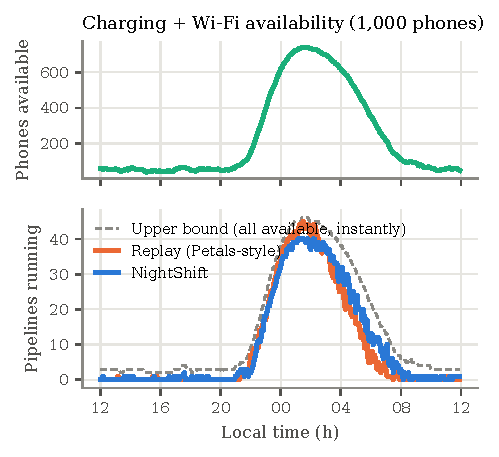
\includegraphics[width=0.8\linewidth]{timeline}
\caption{One simulated day. Top: phones available. Bottom: pipelines running
and an upper bound that assumes instant, perfect placement.}
\label{fig:timeline}
\end{figure}

\paragraph{The pool is a night-time machine} Availability swings from
\MinAvail{} to \PeakAvail{} of 1,000 phones over the day
(Figure~\ref{fig:timeline}), and \NightSharePct\% of tokens are produced
between 22:00 and 08:00. Daytime sessions are short and scattered, so few
complete 16-phone pipelines form. A phone pool is best treated as a batch
system that drains a queue overnight.

\begin{figure}[t]
\centering
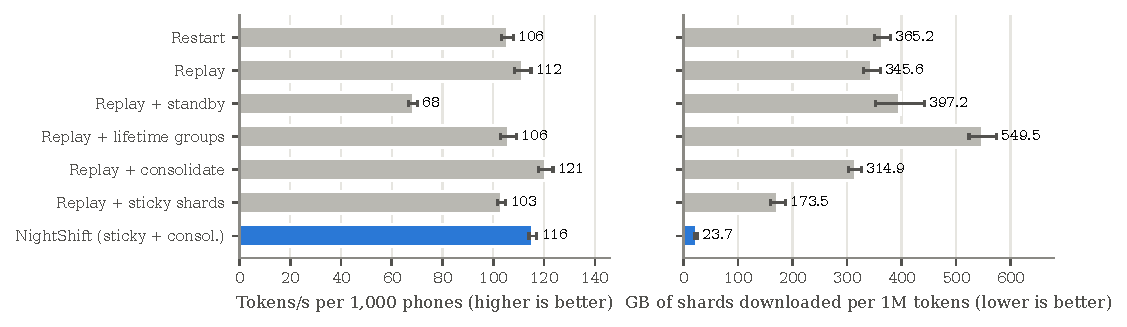
\includegraphics[width=\linewidth]{policies}
\caption{Throughput and data downloaded (shards, dark; repair activations,
light) of the ten policies (1,000 phones, mean $\pm$ s.d.\ over \Seeds{}
seeds). The last four rows add NightShift's parts one at a time.}
\label{fig:policies}
\end{figure}

\paragraph{Moving shards, not lost work, is the cost of churn}
Figure~\ref{fig:policies} compares the policies. Restart differs from replay by
only \RestartVsReplayPct\% ($\pm$\CIRepRestartPct\%, 95\% CI), so little
computation is lost to departures. What separates the policies is data
movement. Replay already prefers phones that hold the needed block, yet the
pool downloads \GBReplay\,GB per million tokens, of which \ShardReplay\,GB are
shards. Matching cached phones across the whole idle pool when forming
pipelines (cache-aware) helps less than one would expect, to \GBCA\,GB. As
Section~\ref{sec:model} shows, a phone that served one block last time is
equally likely to be needed for any of the other fifteen next time, and at a
given moment the few idle phones seldom hold the right one; a serving phone
still downloads about \PhoneGBCA\,GB a day, enough to make a volunteer's data
plan the binding constraint.

\paragraph{NightShift} NightShift downloads \GBNS\,GB per million tokens:
\GBRatio$\times$ less than replay, \GBRatioCA$\times$ less than cache-aware and
\GBRatioConsol$\times$ less than consolidation; for shards alone the reduction
against replay is \ShardRatio$\times$. A serving phone downloads about
\PhoneGBNS\,GB a day instead of \PhoneGBReplay\,GB. Its throughput is \TputNS{}
tokens/s per 1,000 phones against \TputReplay{} for replay, a paired difference
of \DiffRepNS{} $\pm$ \CIRepNS, which is not significant. The best baseline,
consolidation, is faster: \TputConsol{} tokens/s, a paired difference of
\DiffConsNS{} $\pm$ \CIConsNS{} tokens/s, so NightShift is
\NSbehindConsolPct\% behind it at this pool size. NightShift suffers
\FailDropPct\% fewer stage failures than replay, and its stages spend
\UsefulNS\% of their time computing rather than waiting, against
\UsefulReplay\%. The trade is therefore \NSbehindConsolPct\% of throughput
against the best baseline at 1,000 phones for a large cut in the data
volunteers must download.

\paragraph{The ablation: the wait and consolidation need each other} Giving
each phone a home block and making vacant stages wait for it (\emph{wait})
cuts traffic only to \GBWait\,GB and changes throughput by \DiffRepWait{}
$\pm$ \CIRepWait{} tokens/s against replay: in the morning, stages wait for
home-block phones that have left for the day. Adding lifetime grouping changes
little (\TputSticky{} tokens/s, \GBSticky\,GB). Adding consolidation but no
wait (\emph{NightShift without the wait}) recovers some throughput but keeps
traffic at \GBNSNoWait\,GB, because every vacancy still triggers a download.
Only together does the design work: consolidation supplies home-block phones
from dissolved pipelines, so the wait is usually short and usually rewarded
(Equation~\ref{eq:fallback}). Lifetime grouping alone, without home blocks, is
worse than random (\TputLifetime{} tokens/s, \GBLifetime\,GB), because ranking
phones by predicted stay overrides any chance of reusing a cached block.

\paragraph{Standbys are a bad trade on phones} One standby per stage cuts
throughput by \StandbyDropPct\%: it removes half of the pool from service to
protect pipelines whose expected lifetime, at night, is hours. Redundancy pays
off when failures are frequent relative to the cost of idling capacity, as for
preemptible cloud GPUs~\citep{bamboo,oobleck}, but not here.

\begin{figure}[t]
\centering
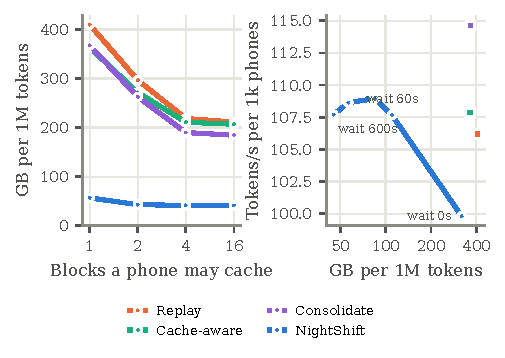
\includegraphics[width=\linewidth]{tradeoff}
\caption{Left: traffic when each phone may cache more blocks. Right: throughput
against traffic; NightShift's wait time (0--600\,s) traces a trade-off, squares
are baselines.}
\label{fig:tradeoff}
\end{figure}

\paragraph{Larger caches do not close the gap} One might expect the baselines
to catch up if phones simply kept more blocks in flash.
Figure~\ref{fig:tradeoff} (left) varies the cache from one block to all 16 (the
whole 40\,GB model). Baseline traffic roughly halves (replay
\CacheFullReplay, cache-aware \CacheFullCA, consolidation \CacheFullConsol\,GB
per million tokens with a full cache) while NightShift falls to
\CacheFullNS\,GB, still \CacheFullRatioCA$\times$ less than cache-aware. With
a full cache no shard is ever downloaded after onboarding, so the remaining
traffic is repair activations, which NightShift's fewer failures also reduce.

\paragraph{The wait is a knob} Figure~\ref{fig:tradeoff} (right) varies how
long a vacant stage waits for a home-block phone. With no wait, NightShift is
the no-wait ablation above (\WaitZeroTput{} tokens/s, \WaitZeroGB\,GB). A
60-second wait already gives \WaitSixtyTput{} tokens/s at \WaitSixtyGB\,GB, and
600\,s gives \WaitTenTput{} tokens/s at \WaitTenGB\,GB. Throughput is nearly
flat beyond a minute while traffic keeps falling, so an operator can choose
the point that suits the volunteers' data plans, using
Equation~(\ref{eq:fallback}) as a guide.

\begin{figure}[t]
\centering
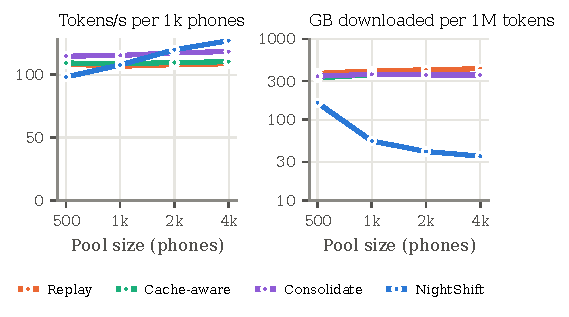
\includegraphics[width=\linewidth]{scale}
\caption{NightShift improves with pool size; the baselines do not. Traffic
(shards plus activations) is on a logarithmic scale.}
\label{fig:scale}
\end{figure}

\paragraph{NightShift gets better with scale} With more phones, each block has
more idle owners to choose from, so a vacant stage rarely waits long or falls
back to a download (Figure~\ref{fig:scale}). From 500 to 4,000 phones,
NightShift's throughput rises from \SwPoolLoNS{} to \SwPoolHiNS{} tokens/s per
1,000 phones and its traffic falls from \PoolSmallGBNS{} to
\PoolLargeGBNS\,GB per million tokens, while the baselines stay roughly flat
(replay \SwPoolLoReplay{} to \SwPoolHiReplay, consolidation \SwPoolLoConsol{}
to \SwPoolHiConsol). At 500 phones NightShift is worse: \PoolSmallGainPct\%
against replay and \PoolSmallVsConsolPct\% against consolidation, with only
\PoolSmallGBRatio$\times$ less traffic. At 4,000 it is \PoolLargeGainPct\%
against replay and \PoolLargeVsConsolPct\% against consolidation, with
\PoolLargeGBRatio$\times$ less traffic than replay and
\PoolLargeGBRatioCA$\times$ less than cache-aware. A deployment worth building
would have far more than 4,000 phones, but we have not simulated beyond that,
and a large pool would likely be split by region (below), which brings each
region back toward smaller pools.

\begin{figure}[t]
\centering
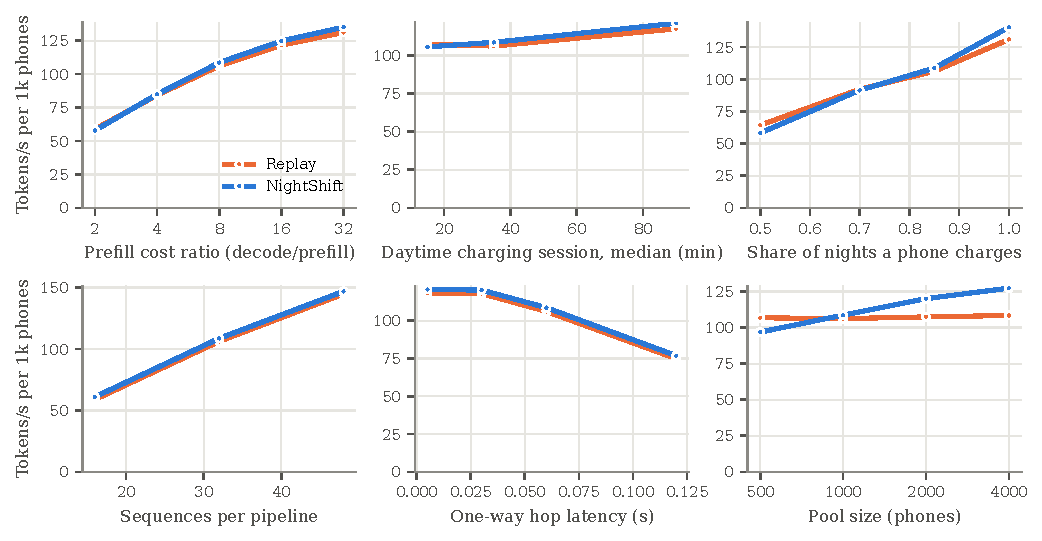
\includegraphics[width=\linewidth]{sweeps}
\caption{Sensitivity of throughput to the main assumptions, replay vs.\
NightShift (1,000 phones unless the panel varies pool size; mean of \Seeds{}
seeds).}
\label{fig:sweeps}
\end{figure}

\paragraph{Sensitivity} Figure~\ref{fig:sweeps} varies one assumption at a
time. Three matter a lot. The share of nights a phone charges moves
NightShift's throughput from \SwNightLoNS{} to \SwNightHiNS{} tokens/s per
1,000 phones between 50\% and 100\% of nights (at 50\%, replay is slightly
ahead). The batch size moves it from \SwBatchLoNS{} (16 sequences) to
\SwBatchHiNS{} (48), because more sequences keep more stages busy; memory for
the KV cache caps this. The cost ratio of decode to prefill moves it from
\SwPrefillLoNS{} (ratio 2) to \SwPrefillHiNS{} (ratio 32): the prompt of every
batch is processed once per stage, and each repair recomputes the cache of all
tokens so far. Raising the median daytime session from 15 to 90 minutes
changes throughput by \DayGainPct\% (\SwDayDurLoNS{} to \SwDayDurHiNS), less
than the night share moves it, confirming that the night carries the system.
Hop latency sets the time per output token once the trip is longer than 16
times the slowest stage (Figure~\ref{fig:latency}: \LatLAN\,s at 5\,ms, where
the slowest stage sets it, \LatWAN\,s at 60\,ms, \LatSlow\,s at 120\,ms), and
with it throughput (\SwHopLoNS{} to \SwHopHiNS). Grouping pipelines by region,
so that hops stay short, is therefore worth more than the scheduling
differences we study. Across every setting we tried, NightShift downloads
\GBRatioMin--\GBRatioMax$\times$ less than replay, the low end at 500 phones.
Its throughput differs from replay's by \SwGainMin\% to \SwGainMax\%: it is
behind at 500 phones (\PoolSmallGainPct\%) and at 50\% of nights
(\SwNightLoGainPct\%), ahead at 2,000 and 4,000 phones (\PoolLargeGainPct\% at
4,000) and when every phone charges every night (\SwNightHiGainPct\%), and
within about 4\% elsewhere.

\begin{figure}[t]
\centering
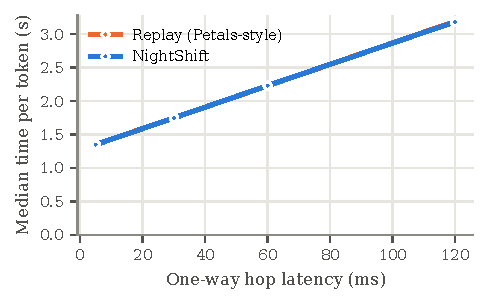
\includegraphics[width=0.75\linewidth]{latency}
\caption{Median time per output token against one-way hop latency.}
\label{fig:latency}
\end{figure}

%% ---------------------------------------------------------------------------
\section{Measurements on real phones}
\label{sec:measure}

The results above rest on assumed parameters. This section reports
measurements that replace them, made with the released benchmark kit, and
checks the simulator's timing model against a real pipeline of phones.

\paragraph{Setup} \Pending{Study A: list of phones (model, SoC, RAM, Android
version), the 8B model and quantisation used, the network (same Wi-Fi /
different homes), dates, and how many runs per measurement.} Compute is
measured with llama.cpp~\citep{llamacpp} on Android (Termux): decode and
prefill speed, the cost of batching 1--8 sequences, sustained speed over
30 minutes, and battery draw. Per-layer time is scaled to the 70B layer by
bytes of weights read, since phone decode is memory-bandwidth bound. The
pipeline test runs the 8B model split over 1--4 phones with llama.cpp's RPC
backend.

\paragraph{Per-phone compute} \Pending{Table: measured ms per layer (70B-scaled)
per phone vs.\ the assumed 10--30\,ms; measured batching cost factor vs.\ the
assumed $1+0.1(b-1)$; measured prefill-to-decode cost ratio vs.\ the assumed
1/8.}

\paragraph{Sustained performance and heat} \Pending{Figure: tokens/s and
battery temperature over a 30-minute run per phone; the ratio of sustained to
initial speed; measured power while computing and while idle-but-plugged vs.\
the assumed 4\,W / 1\,W.}

\paragraph{Network} \Pending{Measured one-way latency and throughput between two
phones on the same Wi-Fi and in different homes, vs.\ the assumed 5\,ms and
60\,ms hops and 50\,Mbit/s downlink.}

\paragraph{Timing model check} For a pipeline of $p$ phones running the 8B
model, Equation~(\ref{eq:ttok}) predicts the time per token from the measured
per-stage times and hop latency. \Pending{Table: predicted vs.\ measured time
per token for $p=1\ldots4$ and the relative error; target below 15\%.}

\paragraph{Re-running the experiments} \Pending{Rerun every experiment with
the measured parameters (PHONESIM\_PARAMS) and report the headline numbers
next to the simulated ones: throughput per 1,000 phones, GB per million tokens
for NightShift and each baseline, and whether the ranking of policies changes.}

\paragraph{Availability} \Pending{Study B, if available: N volunteers' charging
and Wi-Fi logs over 14 days, the fitted session distributions vs.\ the assumed
ones, and NightShift vs.\ baselines on the real trace. Otherwise state that
availability remains synthetic and cite large published
traces~\citep{yang2021heterogeneity} as the next input.}

%% ---------------------------------------------------------------------------
\section{Security, privacy and integrity}
\label{sec:security}

A pool of strangers' phones is an untrusted platform. We state a threat model,
what NightShift does and does not address, and what deployment would need.

\paragraph{Threat model} The coordinator is trusted and run by the operator.
Phones are run by volunteers, some of whom are curious (they inspect what
passes through their stage), some faulty (they return wrong results because of
bugs, overheating or corrupted weights), and a few malicious (they return
wrong results on purpose, or join many times under different identities, a
Sybil attack~\citep{sybil}). Network links between phones may be observed. We
do not consider attacks on the coordinator itself or denial of service.

\paragraph{Confidentiality of prompts} A stage sees the activations of the
tokens that pass through it, and activations can be inverted to recover their
input: model inversion attacks against split and collaborative
inference~\citep{he2019inversion,splitlearning} reconstruct inputs from
intermediate representations, and the first stage, which sees embeddings, is
the most exposed. Encrypting links protects against observers but not against
the stage itself. Trusted execution environments can hide a computation from
its host~\citep{slalom}, but phone TEEs are not available to ordinary apps for
general computation at this scale. We therefore restrict the design to work
whose inputs are not sensitive: public corpora, synthetic data generation,
benchmark evaluation and similar batch jobs. This is a real limitation, and it
also shapes the market: it excludes most enterprise data.

\paragraph{Integrity of results} A faulty or malicious stage can return wrong
activations, and every later stage and every generated token depends on them.
Three defences exist, at increasing cost. \emph{Spot checks:} the coordinator
recomputes a random sample of stage outputs on trusted hardware or on a second
phone and compares; a phone caught once is excluded, so a cheater with
probability $p$ of being sampled per batch is caught within $1/p$ batches in
expectation. Lightweight fingerprints of the computation, such as
TOPLOC~\citep{toploc}, make the comparison cheap. \emph{Redundant
execution:} BOINC-style replication of each stage on two phones~\citep{boinc}
detects any single fault but halves throughput, which our standby result
suggests is costly. \emph{Proofs:} verifiable inference~\citep{safetynets} and
zero-knowledge proofs for LLMs~\citep{zkllm} give cryptographic guarantees but
are orders of magnitude too slow for phones today. We expect spot checks to be
the right first step, because the work is batch work whose results can be
checked after the fact; Byzantine agreement~\citep{byzantine} is unnecessary
when a trusted coordinator can re-run any stage.

\paragraph{Sybil and free-riding} If volunteers are rewarded, a participant may
register many emulated phones. Hardware attestation of the device and its app,
which both major mobile platforms offer, and rewards paid only for verified
work raise the cost of such attacks. NightShift's home blocks help a little:
a phone's identity is bound to a block it stores, so re-registering forces a
new download that the operator can rate-limit.

\paragraph{Weights} Distributing a model to volunteers means that the weights
leave the operator's control. This is acceptable for openly licensed
models~\citep{llama2,llama3}, which are the realistic first workload, and
rules out proprietary ones unless each phone holds too small a slice to be
useful, which a 2.5\,GB block is not.

%% ---------------------------------------------------------------------------
\section{The owner's side: battery, heat, data and incentives}
\label{sec:owners}

A volunteer system fails if volunteers leave. This section estimates what
NightShift asks of an owner.

\paragraph{Battery wear and heat} Lithium-ion cells age faster at high
temperature and at high states of charge~\citep{vetter2005}, and a phone that
computes while charging overnight is both warm and nearly full. Users care
about battery life and act on it~\citep{ferreira2011,banerjee2007}, so a pool
that shortens battery life will not keep its volunteers. Phones also throttle
under sustained load~\citep{phonethermal}, which lowers a stage's speed over a
night. Three rules limit the harm: compute only after the battery has reached
a set level (charging then mostly tops up), pause when the battery
temperature exceeds a threshold, and stop at a fixed share of the night.
\Pending{Study A: measured battery temperature and power during a 30-minute
run, and the fraction of the night a phone could compute under a 40\,$^\circ$C
cap.} The simulator does not yet model these rules; they would lower
throughput by the fraction of time phones pause.

\paragraph{Electricity} At the assumed 4\,W while computing, a phone that
serves for seven hours uses about 28\,Wh a night, roughly 10\,kWh a year,
which at typical household tariffs costs a few euros a year. This is small for
one owner and should be stated to volunteers plainly.

\paragraph{Data} This is where the design matters most. Under the cache-aware
baseline a serving phone downloads about \PhoneGBCA\,GB a day, a heavy ask of
any volunteer whose home connection has a data cap; under
NightShift it downloads about \PhoneGBNS\,GB, plus one block (2.5\,GB) when it
joins. An operator should still cap each phone's monthly download and let
volunteers set the cap; the wait time $W$ (Figure~\ref{fig:tradeoff}) is the
knob that keeps the pool within those caps.

\paragraph{Incentives} Why would anyone donate their phone's nights? Volunteer
science has relied on altruism and recognition~\citep{anderson2006}, which
works for research but less well for commercial batch work. Incentive
mechanisms designed for federated learning~\citep{zhan2021incentive} pay
participants per contribution, and the same structure fits here: pay per
verified stage-hour, with the payment funded by the discount at which batch
inference is sold. Whether the marginal value of a phone's night exceeds its
owner's costs (wear, data, electricity, attention) is an empirical question
that a pilot with real volunteers would answer. We do not model incentives in
the simulator; NightShift's contribution is to make the data cost small enough
that the question can be asked.

%% ---------------------------------------------------------------------------
\section{Threats to validity}
\label{sec:threats}

\paragraph{Construct validity} Our throughput metric counts output tokens and
ignores the value of the jobs; our traffic metric counts bytes downloaded and
treats all bytes as equal, while a volunteer may mind a download on mobile
data far more than one on home Wi-Fi (we only use phones on Wi-Fi).
Energy per token uses assumed power, not measured power.

\paragraph{Internal validity} The simulator ignores stragglers within a stage,
thermal throttling over a night, Wi-Fi contention in one home, and iOS's
stricter background limits. Downloads are counted and delay the stage that
waits for them, but do not compete with other traffic on a link. Time advances
in 10-second ticks, which coarsens short events. The analytical model of
Section~\ref{sec:model} was built from the simulator's rules, so its agreement
with the simulator checks our understanding of the mechanism, not the
simulator's fidelity to real phones; that is the role of
Section~\ref{sec:measure}. We fixed the policies' timers (300\,s wait, 600\,s
dissolution) before running the sweeps and report the wait sweep rather than
a tuned value.

\paragraph{External validity} Each result comes from one synthetic 24-hour
window per seed after warm-up, from a synthetic availability model; real
traces may have more correlated departures (for example, everyone unplugging
at 07:00 on a weekday) than ours, and different regions and seasons have
different charging habits. We simulate up to 4,000 phones and one model size;
other models change $B$ and every number that depends on it. The phone
population is a mix of RAM classes chosen to resemble mid-range Android
devices, not a measured market share.

\paragraph{Conclusion validity} Policy differences are paired by seed and
reported with 95\% confidence intervals over \Seeds{} seeds; several
throughput differences are within those intervals, and we say so where they
are. We have not corrected for multiple comparisons across the ten policies.

%% ---------------------------------------------------------------------------
\section{Conclusion}
\label{sec:conclusion}

A pool of charging phones can, in principle, run a model far larger than any
phone, but only as an overnight batch system with seconds per output token and
far more memory traffic per token than a GPU. Within that regime, the cost
that matters most to the volunteers is data: replacing leavers moves model
shards, and an analytical model shows why even a cache-aware design moves
several gigabytes per phone per day when phones keep whatever block they
served last. Giving each phone a permanent home block, waiting briefly for a
phone that holds it, and consolidating broken pipelines cut that traffic
\GBRatioBaseMin--\GBRatioBaseMax$\times$ against our baselines in simulation,
at \NSbehindConsolPct\% of throughput against the best of them at 1,000 phones
and a gain at 4,000; standbys hurt. Deployment would further need spot checks
of results, restriction to non-sensitive inputs, limits on heat and data, and
an incentive that covers the owner's costs. The next steps are measurements
with real volunteers over weeks, larger simulated pools split by region, and a
pilot with a small open model.

%% ---------------------------------------------------------------------------
\section*{Data availability}
The simulator, the analytical model, every result file, the figure scripts and
the benchmark kit are available at
\url{https://github.com/aidinb/nightshift-phone-llm} \Pending{and archived at
Zenodo, DOI to be added at release}.

\section*{Declaration of competing interest}
The author declares no known competing financial interests or personal
relationships that could have appeared to influence the work reported in this
paper.

\section*{Funding}
This research did not receive any specific grant from funding agencies in the
public, commercial, or not-for-profit sectors.

\section*{CRediT authorship contribution statement}
\textbf{Aidin Bazarchi:} Conceptualization, Methodology, Software, Formal
analysis, Investigation, Writing -- original draft, Writing -- review \&
editing, Visualization.

\section*{Declaration of generative AI and AI-assisted technologies in the manuscript preparation process}
\Pending{Author to confirm the wording.} During the preparation of this work
the author used an AI assistant to help write and revise the text and the
simulation code. After using this tool, the author reviewed and edited the
content as needed and takes full responsibility for the content of the
published article.

\bibliographystyle{elsarticle-harv}
\bibliography{refs}

\end{document}
